Die Scholl Reaktion ist eine Kupplungsreaktion, bei der zwei Arenmoleküle unter Einfluss eine Lewis-Säure und einer Protonensäure miteinander reagieren. Entwickelt wurde die Methode vom Schweizer Chemiker Roland Heinrich Scholl (1865-1945).
Diese Kondensation kann sowohl intermolekular als auch intramolekular verlaufen. Zum Einsatz kommen Lewis Säuren wir $AlCl_3$ oder auch $MoCl_5$. In der Vergangenheit wurde die Reaktion eher wenig eingesetzt (hohe Umsatztemperaturen, geringe Ausbeuten, stark saure Katalysatoren, viele Nebenprodukte). Aber gerade ihr Einsatz in Kaskadenreaktionen, mit denen man komplexe aromatische Kohlenwasserstoffe oder Graphenstrukturen herstellen kann, machte sie wieder interessant. \cite{[12]}
\section{mögliche Mechanismen der Schollreaktion}
In der Schollreaktion wird die oxidative Aryl-Aryl Kupplungsreaktion von Übergangsmetall-Halogenen beeinflusst. Diese dienen als Lewis-Säure und als Oxidans. Zwei mögliche Mechanismen der Schollreaktion wurden von Nenitzescu und Balaban vorgeschlagen. %ref [13]?
\begin{figure}[!htpb]
\centering
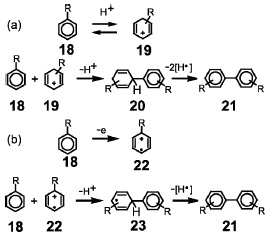
\includegraphics[scale=1]{graphics/Schollreactionmechanismen}
\caption{Menchanismen der Scholl-Reaktion:(a) Arenium-Kation Mechanismus; (b) Radikal-Kation-Mechanismus}
\end{figure}
\\Im Arenium-Kation-Mechanismus wird ein aromatisches Molekül protoniert und der resultierende elektrophilische $\sigma$ Komplex reagiert mit einem anderen aromatischen Kern um einen neue Kohlenstoff-Kohlenstoff-Bindung zu knüpfen. Deprotonierung ergibt das Zwischenprodukt und Dehydrogenierung erzeugt Aromatizität.
\\Im Radikal-Kationen-Mechanismus wird zuerst ein radikales Kation bei einer Ein-Elektronen-Oxidation des Startmaterials gebildet. Dann wird eine C-C-Verknüpfung mit einer aromatischen Gruppe geformt. Deprotonierung und der Verlust eines Wasserstoff-Atoms folgen. Ein arylisch radikalisches Kation wird unter oxidierenden Bedingungen wird zuerst gebildet. Wenn PAHs mit Lewis Säure oder konzentrierte Schwefelsäure behandelt werden, ergeben sich paramagnetischen Lösungen. Deshalb könnten radikale Kationen bei der Schollreaktion entstehen.\cite{[13]}
\section{oxidative Kupplung mit MoCl$_5$}
$MoCl_5$ ist ein schwarzer polymorpher kristalliner Feststoff, der luft- und feuchtigkeitsempfindlich ist und deshalb in inerter Atmosphäre aufbewahrt wird. Das koordinativ ungesättigte $MoCl_5$ ist essentiell für elektrophile Anwendungen. Chlorierte Lösungsmittel, wie Dichlormethan, werden als Reaktionsmedium empfohlen.
\\Bei der Herstellung von hexa-peri-hexabenzocoronen aus hexaphenyl-benzen liefert die Zugabe von $MoCl_5$ die besten Resultate. Diese Reaktion wird später näher erklärt.
Bei der oxidativen Zyklisierung von ortho-terphenylen mit $MoCl_5$ ist das Substitutionsmuster am wichtigsten.  Zumindest eine Donorfunktion soll para zum neu geformten Band stehen, weil sonst kein Produkt entsteht. \cite{14}
\begin{figure}[htpb!]
\centering
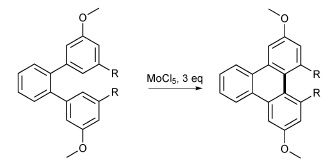
\includegraphics[scale=0.5]{graphics/Scholltriterpene}
\caption{Schollreaktion zu Triphenylen}
\end{figure}

\section{Herstellung von polycyclischen Kohlenwasserstoffen}
\begin{figure}[htpb!]
\centering
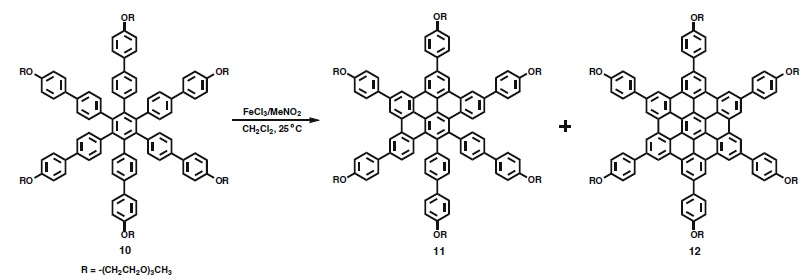
\includegraphics[scale=0.8]{graphics/Schollreactionhbc}
\caption{Synthese von hexaphenyl-1/2HBC und hexaphenyl HBC }
\end{figure}
Hexa peri-hexabenzocoronen(HBC) sind eine Klasse von Polycyclischen Kohlenwasserstoffen, die man als scheibenförmige Strukturen beschreiben kann.  Aus Hexaphenylbenzen kann man mittels Scholl-Reaktion unter Verwendung von $CuCl_2$/$AlCl_3$/$CS_2$ oder $FeCl_3$/$CH_3NO_2$ HBC-Moleküle herstellen. Die Aryl-Aryl dehydrogenische Kupplungsreaktion erfolgt in getrennten Schritten intramolekular mit vier neuen Kohlenstoff-Kohlenstoff-Bindungen in Ausbeute von 10\%. Das ist die einzige isolierte Intermediat einer Schollkondensation eines Hexaphenylbenzen-Vorläufers. Zwei teilweise fusionierte Reaktionsmediate wurden durch Schollkondensation aus einer Kohlenstoff-Oligophenyl-Vorgänger hergestellt. Sterische Hinderung und die Stabilität des Radikalkations bevorzugen diese Formation. Aus pyrimidinhältigen Edukten kann kein HBC hergestellt werden, weil der metallische Katalysator möglicherweise mit dem Substrat reagiert und die Schollreaktion am halben Weg eliminiert. So konnte kein HBC aus einem pyrimidinhältigen Edukt hergestellt werden. Nur richtig designete Hexaphenylbenzen-Vorgänger können eine Schollkondensation eingehen um alkoxy-Substituierte HBCs herzustellen. \cite{[15]}

